\chapter{Detector Testing}
The last step of manufacturing is to test the electrical properties of the detector and evaluate whether it is functioning properly or not.
Several properties must be analyzed in order to determine the quality of the detector; the first of which is leakage current.
In order for the detector to work properly, it must function as a basic capacitor.
If current can flow while the detector has applied voltage, then the amorphous germanium layer is not properly blocking holes and electrons which means the detector will not function.
Thus, a measure of leakage current is a necessary initial step to analyze if the detector will work at all.

If the leakage current is tested and determined to be of an acceptable level (on the order of a few picoamps or less), testing can proceed.
The next property measured is the detector capacitance.
This measurement is made using an injected pulsar and can also determine the depletion voltage of the detector.
The detector capacitance and depletion voltage can also give an accurate measurement for the impurity concentration of the germanium.
Finally the detector spectrum is measured using several radioactive sources such as cobalt 60 and cesium 137.
From this spectrum, the energy resolution of the detector can be determined and thus the overall quality.

All of these measurement must be taken while the detector is at cryogenic temperatures.
They also require the integration of several pieces of electronics that must be easily interchanged to make the different measurements.
The cryostat used at USD is shown in Figure \ref{fig:cryostat-whole}.
In the figure, the black cords coming into the base on the right and left side are a mix of high voltage and signal cables.
The flex tube coming into the middle is a vacuum tube.
The large black cylinder on top is the chicken feeder style liquid nitrogen dewar.
The metal cylinder at the base is where the detector sits.
\begin{figure}[htpb]
\centering
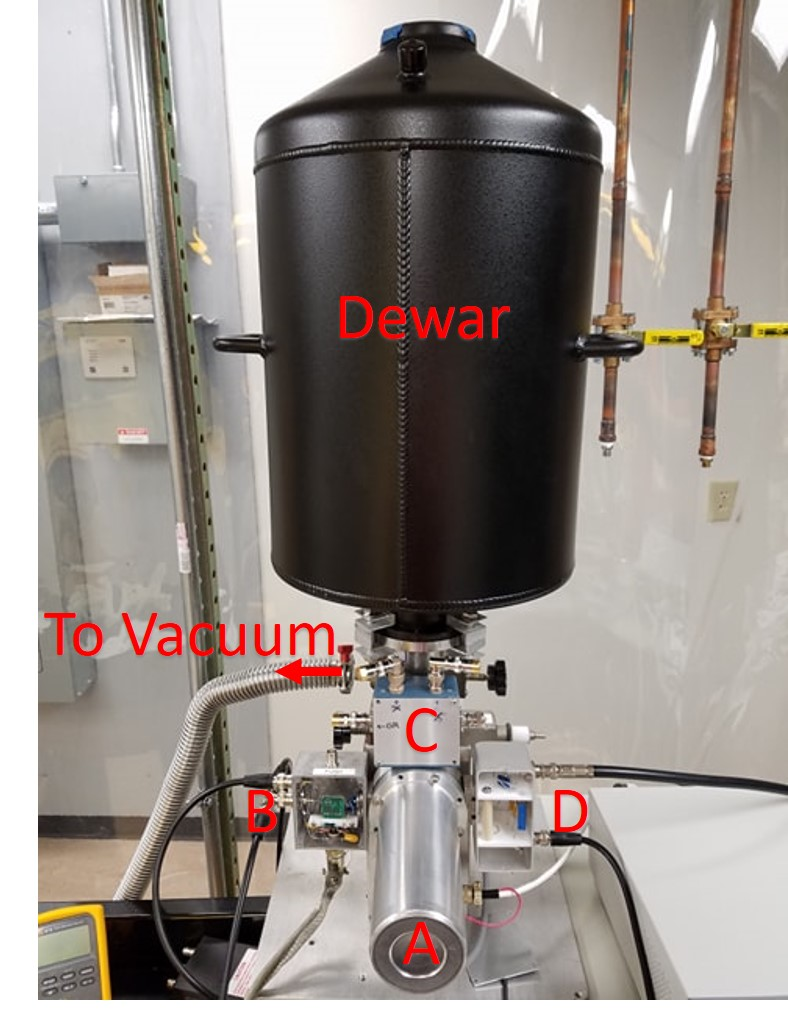
\includegraphics[width=\textwidth]{cryostat-whole}
  \caption{Cryostat system used for detector calibration.A) Detector housing. B) preamplifier and signal output housing. C) Optional detector outputs. D) HV and pulsar input  and HV filter.}
\label{fig:cryostat-whole}
\end{figure}

\section{Detector Cryostat}
All germanium detector cryostats have one thing in common: they must be under vacuum.
The detector itself is mounted on some surface which is covered with a metal cap.
The air is then vacuumed from the enclosure and the detector is able to be efficiently cooled to under 100K.
The method of how the detector is cooled is what varies among different cryostat designs.

Figure \ref{fig:cryostats} shows two types of cryostat designs.
The left side of the figure depicts a cryostat with a cooling finger design.
Typically the detector is in thermal contact with a long metal rod that is submerged in liquid nitrogen.
The rod will eventually reach thermal equilibrium with the liquid nitrogen and is able to then able cool the detector.
\begin{figure}[htpb]
\centering
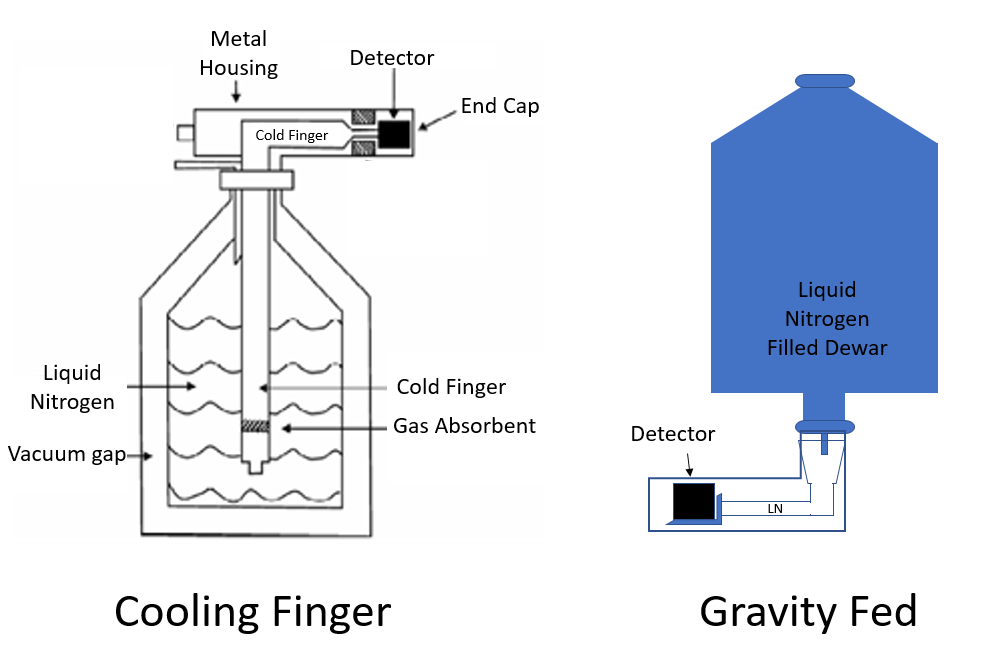
\includegraphics[width=\textwidth]{cryostats}
\caption{Two different cryostat designs}
\label{fig:cryostats}
\end{figure}
The right side of Figure \ref{fig:cryostats} depicts another cryostat that is gravity fed.
Liquid nitrogen is added to a Dewar that sits on top of the detector housing.
Liquid nitrogen can then fill tubes that are connected to the stage holding the detector.
The stage will then reach equilibrium with the liquid nitrogen and cool the detector.

Both designs come with advantages and disadvantages.
The cold finger design is widely used commercially due to its simple design and adaptability to fit many Dewars.
However, the cold finger has draw backs in the minimum temperature that the cryostat can reach.
Portions of the cold finger in direct contact with LN can reach LN temperature, however, points out of the nitrogen will have a temperature gradient that increases along the shaft.
Thus the detector itself will usually be 20 to 30 degrees above that of liquid nitrogen.
The cooling itself is also quite slow with the cold finger method and it can take half a day to cool down.
\begin{figure}[htpb]
\centering
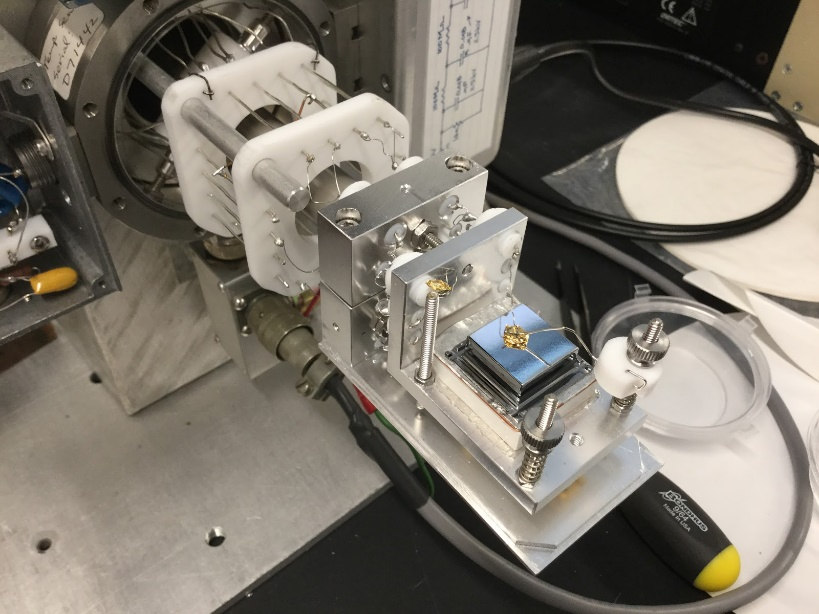
\includegraphics[width=0.8\textwidth]{inner-cryostat}
\caption{}
\label{fig:inner-cryostat}
\end{figure}
The gravity fed design has an advantage that the liquid nitrogen fills the L shaped tube which directly connects to the detector stage.
This results in the detector being much closer to LN  and thus LN temperatures.
The detector can also be relatively quickly cooled down, reaching 80 Kelvin in approximately four hours.

As shown in Figure \ref{fig:cryostat-whole}, the cryostat used at USD for detector characterization and testing is of the gravity fed design.
This particular cryostat was custom designed and manufactured at LBNL.
It has the ability to measure and control the temperature of the germanium detector through the use of a thermistor and heater resistor.
Removing the aluminum can on the front of the detector reveals the inner detector along with the cooling structure as shown in Figure \ref{fig:inner-cryostat}.
Here the detector can be seen as the top hat shaped crystal with a gold foil covered contact placed on the top surface.
Several wires can also be seen leading to the external electronics and circuitry.

A cold finger design is easier for the user since all one has to do is dip the cold finger attached to the detector assembly into LN, however it is hard to open the housing or not allowed.
The gravity fed design has a detector housing that is designed to be opened but the user is responsible for vacuum which makes it nice for research.
Figure \ref{fig:cryostat-whole} shows a view of the cryostat used at USD with the attached input boxes, vacuum tube, and the interface between the cryostat and gravity fed Dewar.
\begin{figure}[htpb]
\centering
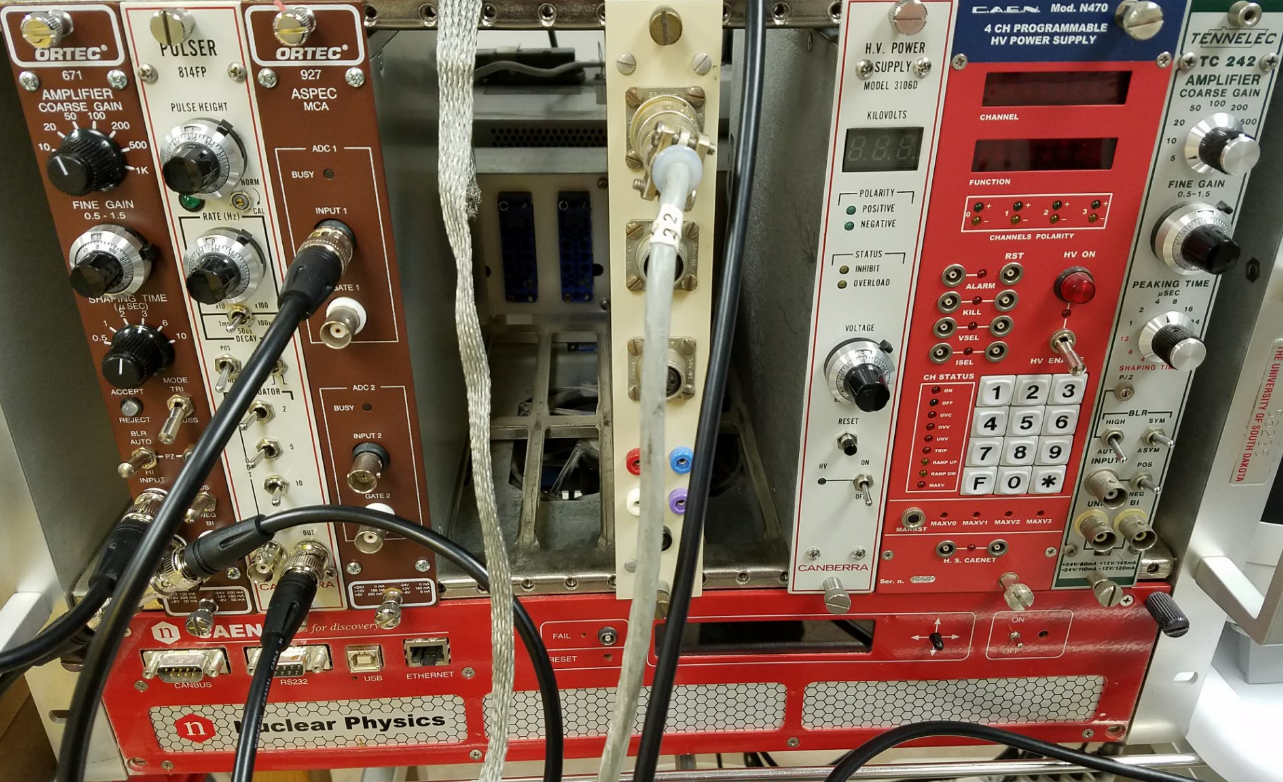
\includegraphics[width=\textwidth]{crate}
\caption{The electronics crate used in detector characterization. From left to right: Ortec shaping amplifier, Canberra pulsar, Ortec ASPEC multi channel analyzer, preamplifier power supply, Canberra HV supply, CAEN HV supply, Tennelec shaping amplifier}
\label{fig:crate}
\end{figure}

\section{Testing}
In order to prove the validity of the entire detector manufacturing process at USD, a detector of known purity from a commercial vendor was processed and tested.
The detector was named HP50765-1N and was through all steps of processing besides cutting which was done by Mark Amman at LBNL.
The first step in detector testing is to measure the leakage current.
If the leakage current is not within a few picoamps to well beyond the depletion voltage, the detector will not function properly
\begin{figure}[htpb]
\centering
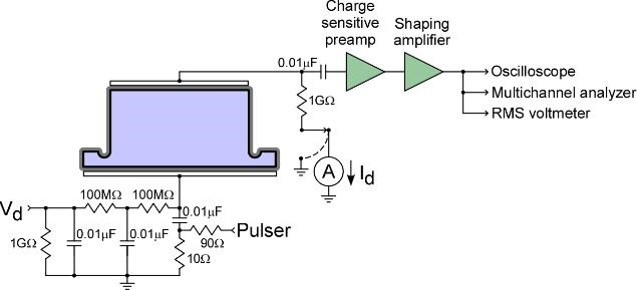
\includegraphics[width=\textwidth]{outline}
\caption{Simple circuit diagram of the germanium detector electronics. Courtesy of Mark Amman}
\label{fig:outline}
\end{figure}
Figure \ref{fig:outline} shows the circuit diagram of the detector and attached electronics inside of the cryostat and electronics housing.
During the first test of a detector, the leakage current is measured with the preamplifier removed so the only avenue for current is out over the 1G$\Omega$ resistor.
The leakage current typically seen during measurement is on the order of a few picoamps.
This low current requires special equipment to be measured.
At USD, a combination of a transimpedance amplifier and multimeter are used.
The transimpedance amplifier takes the current and converts it to a voltage which can then be read out and recorded via a multimeter.
\begin{figure}[htpb]
\centering
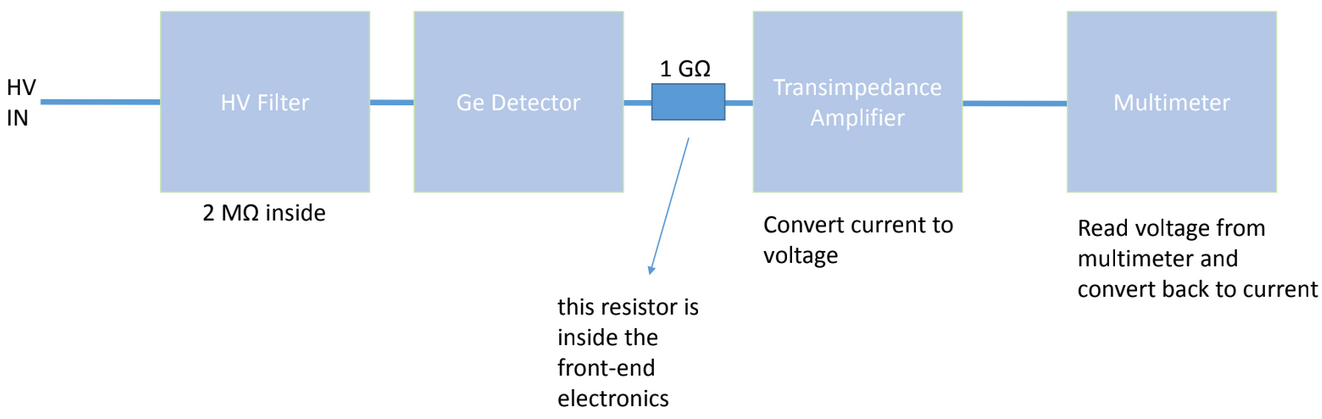
\includegraphics[width=\textwidth]{leakage-measurement}
\caption{Setup diagram for leakage current measurement}
\label{fig:leakage-measurement}
\end{figure}

To begin the testing, detector HP50765-1N was loaded into the cryostat and then cooled down to 79K at which temperature the measurements take place.
\begin{figure}[htpb]
\centering
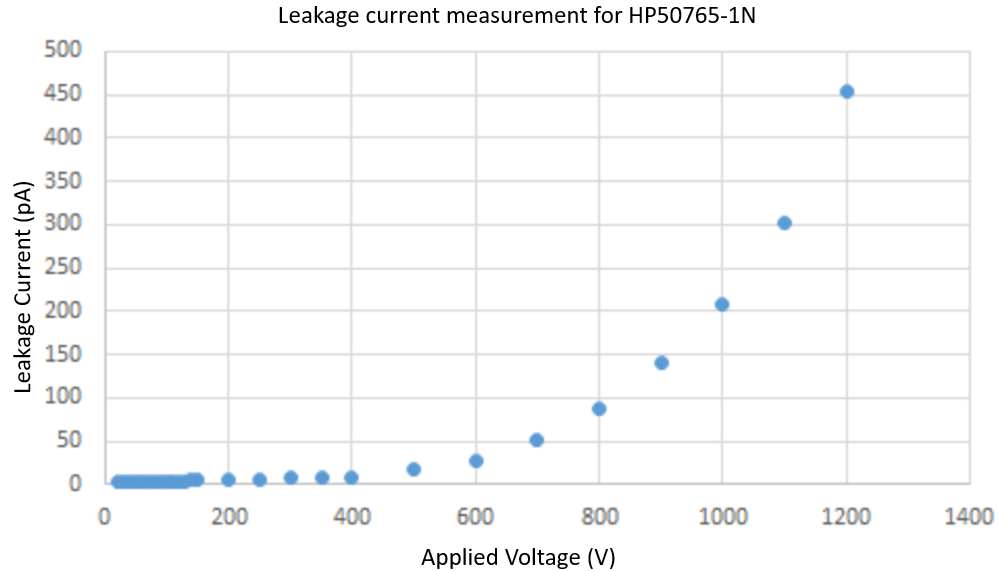
\includegraphics[width=\textwidth]{leakage-test}
\caption{graph of leakage current vs applied voltage}
\label{fig:leakage-test}
\end{figure}
Figure \ref{fig:leakage-test} shows the plot of leakage current vs applied voltage.
The plot shows a stable leakage current of only a few picoamps until around 500 volts where the current begins to rise.
The initial stability of the leakage current shows that the detector contacts are working but the rise means that they are far from perfect.
A good detector should be able to have an applied voltage of several thousand volts before breaking down.

The next step of detector testing is to measure the capacitance
Capacitance measurements involve the use of an injected pulsar of known magnitude.
Pulses are sent to the detector that mimic that of a signal.
As the voltage across the detector is changed, the magnitude of the pulsar will change until the detector reaches its depletion voltage.
The height of this pulsar at depletion voltage can be used to determine the detector capacitance based on the formula:
\begin{align*}
C_d=\frac{Q}{V}=\frac{\frac{E\times 1.6\times 10^{-19}}{2.96ev}}{v(mV)\times \frac{8}{125}}
\end{align*}
where E is the pulsar energy and v(mV) is the pulsar output voltage from the oscilloscope

\begin{figure}[htpb]
\centering
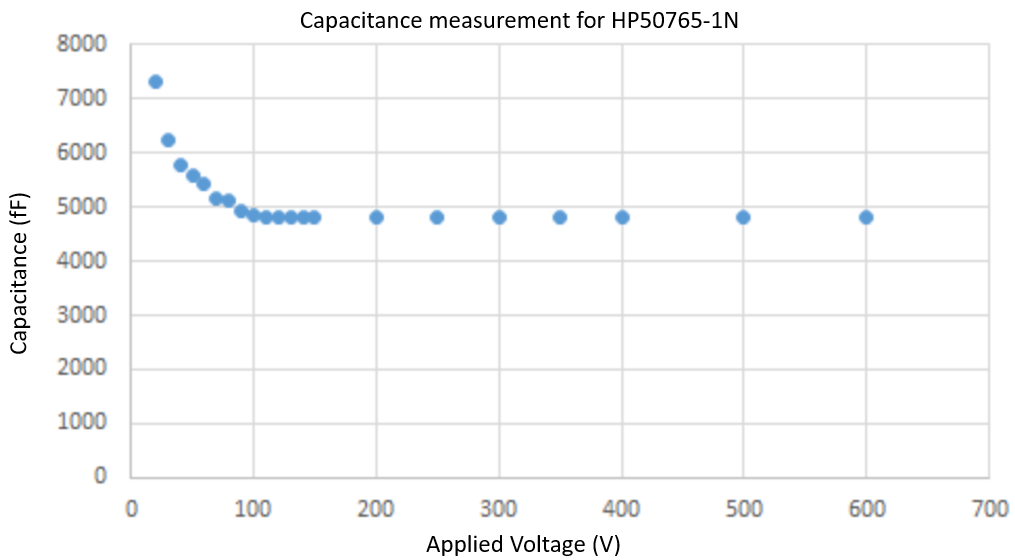
\includegraphics[width=\textwidth]{capacitance-test}
\caption{Plot of detector capacitance vs applied voltage}
\label{fig:capacitance-test}
\end{figure}
Figure \ref{fig:capacitance-test} shows a plot of the detector capacitance vs applied voltage.
As mentioned earlier, the capacitance test can also be a rough test of determining depletion voltage and thus detector purity.
For HP50765-1N, the detector reached a stable capacitance value, and thus depleted, at around 100 volts.
This low depletion voltage means the detector is made of extremely pure material, on the order of $10^{9}cm^{-3}$

\begin{figure}[htpb]
\centering
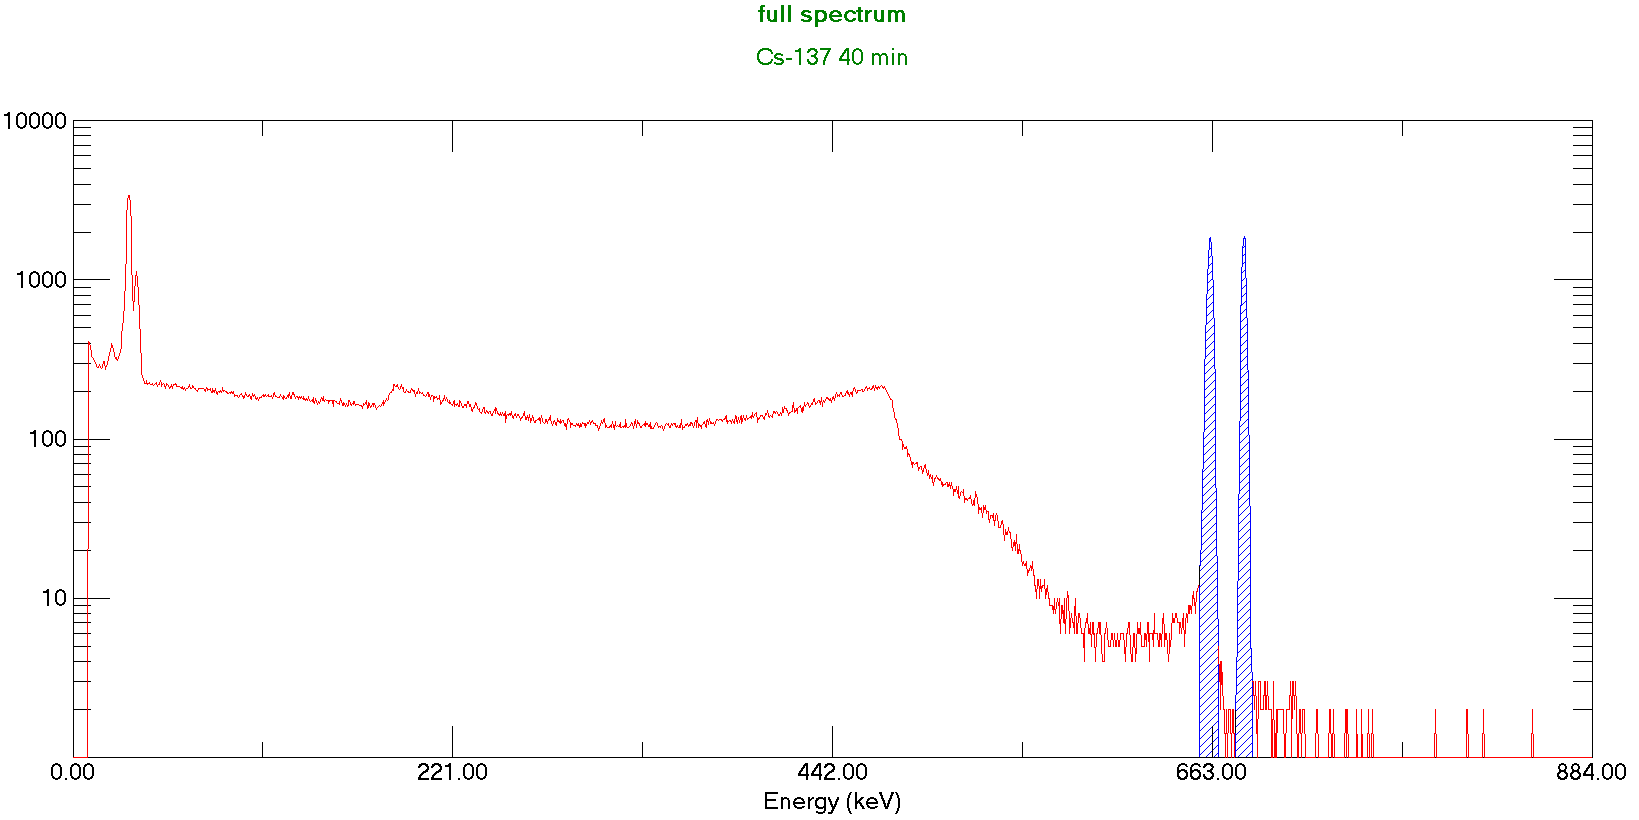
\includegraphics[width=\textwidth]{cs-137-test}
\caption{Spectrum obtained from detector NI with Cs 137 and pulsar peaks highlighted in blue. x-axis is counts}
\label{fig:cs-137-test}
\end{figure}
Since the detector passed both the leakage current and capacitance tests, it can be exposed to a radioactive source and a spectrum can be obtained.
For this test, the detector was exposed to a Cesium 137 source as well as continuous pulsar injection.
Figure \ref{fig:cs-137-test} shows the spectrum after 40 minutes of exposure.
The gamma ray and pulsar peaks are highlighted in blue.
As mentioned earlier, Cs 137 has a gamma ray peak at 662 keV which matches the spectrum perfectly.
Also shown clearly is the Compton edge and shoulder mentioned in chapter 2.

The energy resolution of the detector can be determined by evaluating the pulsar and 662 keV peak for their width at half of the max point of the distribution.
This is called full-width half max (FWHM) and is a measure of how spread out the energy distribution of the peak is.
Perfect energy resolution would result in a straight line while spreading of the peak results in lower energy resolution.
The Cs 137 peak at 662 keV for detector HP50765-1N has a FWHM of the 2.83 as shown in Figure \ref{fig:662-pulsar} which is similar to standard germanium detectors.
\begin{figure}[htpb]
\centering
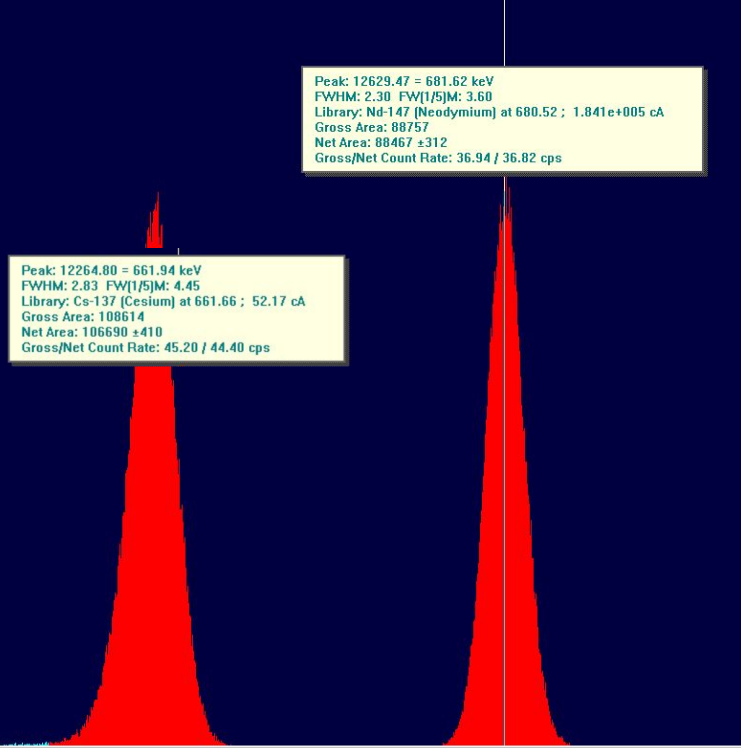
\includegraphics[width=0.8\textwidth]{662-pulsar}
\caption{Cs-137 and injected pulsar peak information with FWHM}
\label{fig:662-pulsar}
\end{figure}


